\newpage

\section{Pythagorean Theorem}

\begin{teachingnote}
Before problem 1, ask:  ``State the Pythagorean Theorem.''  Give students about a minute to write something down.  Many students will write only, ``$a^2 + b^2 = c^2$.''  Then in whole class discussion, draw out the missing pieces:  (1) that $a$, $b$, and $c$ are side lengths of a triangle;  (2) that the triangle is a right triangle; and (3) that $c$ is the length of the hypotenuse.  Then, the class decision can be as follows: 
 
\begin{quote}\textbf{Pythagorean Theorem:}  Suppose a triangle has side lengths $a$, $b$, and $c$.  If the triangle is right with hypotenuse $c$, then $a^2 + b^2 = c^2$. 
\end{quote}
The advantage of this phrasing is that it paves the way for a clear statement of a converse (below).   

Some students will use only the left picture and algebra (i.e., the distributive property) to get the desired result.  The advantage of both pictures is that algebra is not necessary, as the right picture provides the distributive property via rearranging the pieces.  

Once they have proven the Pythagorean Theorem for the particular triangle as drawn, ask, ``How do we know it will work for any triangle?''  The conceptual leap is that the reasoning is exactly the same.  

The term \emph{converse} may need to be introduced.  Perhaps include an example of a true statement with a false converse (e.g., about vertical angles, or about divisibility by 4 and even).  

\begin{quote}
\textbf{Converse of the Pythagorean Theorem:}  Suppose a triangle has side lengths $a$, $b$, and $c$.  If $a^2 + b^2 = c^2$, then the triangle is right with hypotenuse $c$. 
\end{quote}

For the proof, construct a separate right triangle with legs of length $a$ and $b$ and hypotenuse $d$.  By the (forward direction) of the Pythagorean Theorem, $a^2+b^2=d^2$.  (For students who find it difficult to accept this reasoning, it can help to remind them that a statement and its converse are logically distinct.)  By algebra, $c=d$.  By SSS, the two triangles are congruent, so the original triangle must be right.  

Perhaps add a problem about the history involving Egyptians, ropes, knots, and right angles.  Ask whether it is about the theorem or the converse. 
\end{teachingnote}


\begin{prob}
Give two explanations of how the following picture ``proves''
  the Pythagorean Theorem, one using algebra and one without algebra.\standard{8.G.6} 
\[
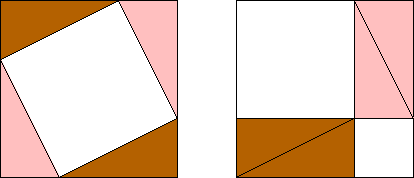
\includegraphics[scale=1.3]{../graphics/pbppyth1.pdf}
\]
\end{prob}
\vfill

\newpage

\begin{prob}
State the converse of the Pythagorean Theorem and prove it.  
\end{prob}

